% Autore= Enrico Salmaso

\subsubsection{UCS 7 - Monitoraggio degli accessi effettuati}
\begin{figure}[h]
	\centering
	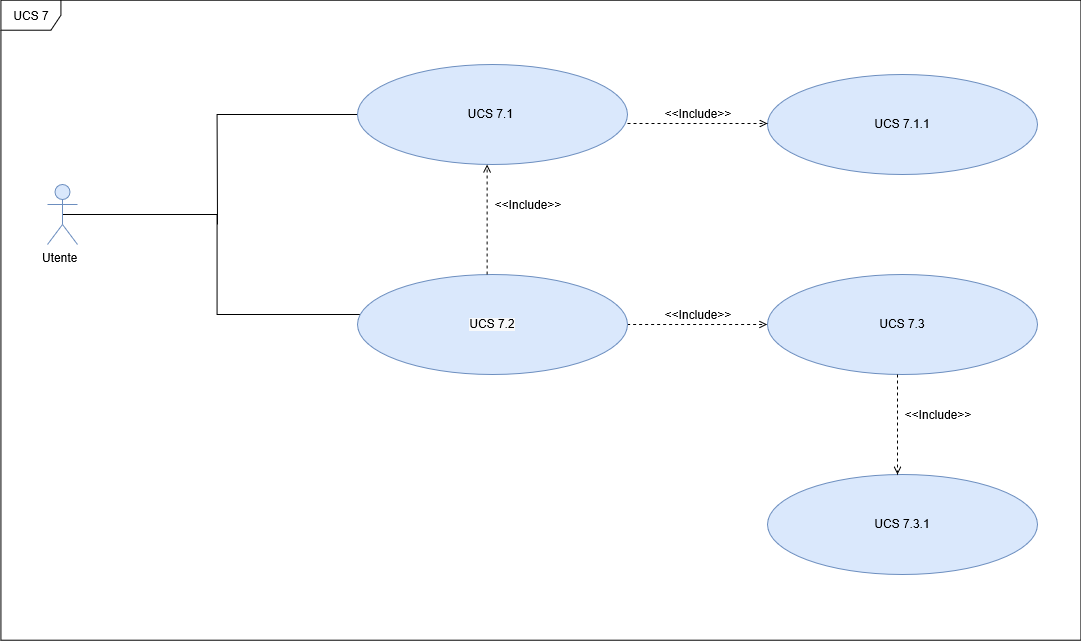
\includegraphics[scale=0.3]{sezioni/UseCase/Immagini/UCS7.png}
	\caption{UCS 7 - Monitoraggio degli accessi effettuati}
\end{figure}

\begin{itemize}
\item \textbf{Attori primari:} Amministratore visualizzatore
\item \textbf{Precondizione:} L'amministratore dispone di almeno un'organizzazione.
\item \textbf{Postcondizione:} L'amministratore ha monitorato gli accessi effettuati dagli utenti riconosciuti.
\item \textbf{Scenario principale:} L'amministratore, dopo aver selezionato l'organizzazione, accede alla funzionalità di visualizzazione della lista degli accessi per monitorare gli utenti.
\item \textbf{Flusso di eventi:} 
\begin{enumerate}
	\item L'amministratore ha selezionato l'organizzazione [UCS 3];
	\item L'amministrazione seleziona la funzionalità di visualizzazione della lista degli accessi;
	\item L'amministrazione può visualizzare gli accessi effettuati da un utente riconosciuto [UCS 7.1].
\end{enumerate}
\end{itemize}

\subsubsection{UCS 7.1 - Visualizzazione degli accessi effettuati da un utente riconosciuto}
\begin{itemize}
	\item \textbf{Attori primari:} Amministratore visualizzatore
	\item \textbf{Precondizione:} L'amministratore ha effettuato l'accesso alla funzionalità di monitoraggio degli accessi effettuati.
	\item \textbf{Postcondizione:} L'amministratore ha visualizzato una lista con gli accessi di un utente riconosciuto.
	\item \textbf{Scenario principale:} L'amministratore può visualizzare gli accessi effettuati da un utente riconosciuto e ha la possibilità di:
	\begin{itemize}
	\item Tornare indietro al monitoraggio degli accessi di tutti gli utenti [UCS 7.1.1];
	\item Visualizzare gli accessi effettuati in base a una data [UCS 7.2].
	\end{itemize}
	\item \textbf{Flusso di eventi:}
	\begin{enumerate}
	\item L'amministratore seleziona un utente preciso da una lista contente tutti i utenti riconosciuti dell'organizzazione;
	\item L'amministratore visualizza una lista con tutti gli accessi effettuati dall'utente selezionato.
	\end{enumerate}
	\item \textbf{Inclusioni:}
	\begin{itemize}
		\item UCS 7.2 - Visualizzazione degli accessi effettuati da un utente riconosciuto in base a una data.
	\end{itemize}

\end{itemize}

\subsubsection{UCS 7.1.1 - Ritorno al monitoraggio degli accessi}
	\item \textbf{Attori primari:} Amministratore visualizzatore
	\item \textbf{Precondizione:} L'amministratore si trova all'interno della funzionalità di visualizzazione degli accessi effettuati da un utente riconosciuto.
	\item \textbf{Postcondizione:} L'amministratore ha effettuato l'accesso alla funzionalità di monitoraggio degli accessi di tutti gli utenti.
	\item \textbf{Scenario principale:} L'amministratore ha scelto di tornare al monitoraggio di tutti gli utenti.
	\item \textbf{Flusso di eventi:}
    \begin{enumerate}
        \item  L'amministratore seleziona la funzionalità per tornare indietro a monitorare gli accessi di tutti gli utenti.
    \end{enumerate}


\subsubsection{UCS 7.2 - Visualizzazione degli accessi effettuati da un utente riconosciuto in base a una data}
\begin{itemize}
	\item \textbf{Attori primari:} Amministratore visualizzatore
	\item \textbf{Precondizione:} L'amministratore ha selezionato un utente riconosciuto per visualizzarne gli accessi.
	\item \textbf{Postcondizione:} L'amministratore ha inserito una data per filtrare l'elenco degli accessi.
	\item \textbf{Scenario principale:} L'amministratore, dopo aver selezionato la funzionalità di visualizzazione degli accessi in base a una data, potrà inserire una data per ottenere una ricerca più dettagliata degli accessi dell'utente riconosciuto.
	\item \textbf{Flusso di eventi:} 
	\begin{enumerate}
		\item L'amministratore ha scelto la funzionalità di visualizzazione degli accessi in base a una data;
		\item L'amministratore inserirà una data [UCS 7.2.1].
	\end{enumerate}
	\item \textbf{Inclusioni:}
	\begin{enumerate}
		\item UCS 7.2.1 - Inserimento della data.
	\end{enumerate}
\end{itemize}

\subsubsection{UCS 7.2.1 - Inserimento della data }
\begin{itemize}
	\item \textbf{Attori primari:} Amministratore visualizzatore
	\item \textbf{Precondizione:} L'amministratore deve inserire una data per filtrare l'elenco degli accessi.
	\item \textbf{Postcondizione:} L'amministratore ha inserito la data.
\end{itemize}




